% Options for packages loaded elsewhere
\PassOptionsToPackage{unicode}{hyperref}
\PassOptionsToPackage{hyphens}{url}
%
\documentclass[
  english,
  man, fleqn, noextraspace]{apa6}
\usepackage{lmodern}
\usepackage{amssymb,amsmath}
\usepackage{ifxetex,ifluatex}
\ifnum 0\ifxetex 1\fi\ifluatex 1\fi=0 % if pdftex
  \usepackage[T1]{fontenc}
  \usepackage[utf8]{inputenc}
  \usepackage{textcomp} % provide euro and other symbols
\else % if luatex or xetex
  \usepackage{unicode-math}
  \defaultfontfeatures{Scale=MatchLowercase}
  \defaultfontfeatures[\rmfamily]{Ligatures=TeX,Scale=1}
\fi
% Use upquote if available, for straight quotes in verbatim environments
\IfFileExists{upquote.sty}{\usepackage{upquote}}{}
\IfFileExists{microtype.sty}{% use microtype if available
  \usepackage[]{microtype}
  \UseMicrotypeSet[protrusion]{basicmath} % disable protrusion for tt fonts
}{}
\makeatletter
\@ifundefined{KOMAClassName}{% if non-KOMA class
  \IfFileExists{parskip.sty}{%
    \usepackage{parskip}
  }{% else
    \setlength{\parindent}{0pt}
    \setlength{\parskip}{6pt plus 2pt minus 1pt}}
}{% if KOMA class
  \KOMAoptions{parskip=half}}
\makeatother
\usepackage{xcolor}
\IfFileExists{xurl.sty}{\usepackage{xurl}}{} % add URL line breaks if available
\IfFileExists{bookmark.sty}{\usepackage{bookmark}}{\usepackage{hyperref}}
\hypersetup{
  pdftitle={The title},
  pdfauthor={Joseph F. T. Nese1},
  pdflang={en-EN},
  pdfkeywords={keywords},
  hidelinks,
  pdfcreator={LaTeX via pandoc}}
\urlstyle{same} % disable monospaced font for URLs
\usepackage{graphicx,grffile}
\makeatletter
\def\maxwidth{\ifdim\Gin@nat@width>\linewidth\linewidth\else\Gin@nat@width\fi}
\def\maxheight{\ifdim\Gin@nat@height>\textheight\textheight\else\Gin@nat@height\fi}
\makeatother
% Scale images if necessary, so that they will not overflow the page
% margins by default, and it is still possible to overwrite the defaults
% using explicit options in \includegraphics[width, height, ...]{}
\setkeys{Gin}{width=\maxwidth,height=\maxheight,keepaspectratio}
% Set default figure placement to htbp
\makeatletter
\def\fps@figure{htbp}
\makeatother
\setlength{\emergencystretch}{3em} % prevent overfull lines
\providecommand{\tightlist}{%
  \setlength{\itemsep}{0pt}\setlength{\parskip}{0pt}}
\setcounter{secnumdepth}{-\maxdimen} % remove section numbering
% Make \paragraph and \subparagraph free-standing
\ifx\paragraph\undefined\else
  \let\oldparagraph\paragraph
  \renewcommand{\paragraph}[1]{\oldparagraph{#1}\mbox{}}
\fi
\ifx\subparagraph\undefined\else
  \let\oldsubparagraph\subparagraph
  \renewcommand{\subparagraph}[1]{\oldsubparagraph{#1}\mbox{}}
\fi
% Manuscript styling
\usepackage{upgreek}
\captionsetup{font=singlespacing,justification=justified}

% Table formatting
\usepackage{longtable}
\usepackage{lscape}
% \usepackage[counterclockwise]{rotating}   % Landscape page setup for large tables
\usepackage{multirow}		% Table styling
\usepackage{tabularx}		% Control Column width
\usepackage[flushleft]{threeparttable}	% Allows for three part tables with a specified notes section
\usepackage{threeparttablex}            % Lets threeparttable work with longtable

% Create new environments so endfloat can handle them
% \newenvironment{ltable}
%   {\begin{landscape}\begin{center}\begin{threeparttable}}
%   {\end{threeparttable}\end{center}\end{landscape}}
\newenvironment{lltable}{\begin{landscape}\begin{center}\begin{ThreePartTable}}{\end{ThreePartTable}\end{center}\end{landscape}}

% Enables adjusting longtable caption width to table width
% Solution found at http://golatex.de/longtable-mit-caption-so-breit-wie-die-tabelle-t15767.html
\makeatletter
\newcommand\LastLTentrywidth{1em}
\newlength\longtablewidth
\setlength{\longtablewidth}{1in}
\newcommand{\getlongtablewidth}{\begingroup \ifcsname LT@\roman{LT@tables}\endcsname \global\longtablewidth=0pt \renewcommand{\LT@entry}[2]{\global\advance\longtablewidth by ##2\relax\gdef\LastLTentrywidth{##2}}\@nameuse{LT@\roman{LT@tables}} \fi \endgroup}

% \setlength{\parindent}{0.5in}
% \setlength{\parskip}{0pt plus 0pt minus 0pt}

% \usepackage{etoolbox}
\makeatletter
\patchcmd{\HyOrg@maketitle}
  {\section{\normalfont\normalsize\abstractname}}
  {\section*{\normalfont\normalsize\abstractname}}
  {}{\typeout{Failed to patch abstract.}}
\patchcmd{\HyOrg@maketitle}
  {\section{\protect\normalfont{\@title}}}
  {\section*{\protect\normalfont{\@title}}}
  {}{\typeout{Failed to patch title.}}
\makeatother
\shorttitle{Title}
\keywords{keywords\newline\indent Word count: X}
\DeclareDelayedFloatFlavor{ThreePartTable}{table}
\DeclareDelayedFloatFlavor{lltable}{table}
\DeclareDelayedFloatFlavor*{longtable}{table}
\makeatletter
\renewcommand{\efloat@iwrite}[1]{\immediate\expandafter\protected@write\csname efloat@post#1\endcsname{}}
\makeatother
\usepackage{lineno}

\linenumbers
\usepackage{csquotes}
\raggedbottom
\setlength{\parskip}{0pt}
\ifxetex
  % Load polyglossia as late as possible: uses bidi with RTL langages (e.g. Hebrew, Arabic)
  \usepackage{polyglossia}
  \setmainlanguage[]{english}
\else
  \usepackage[shorthands=off,main=english]{babel}
\fi

\title{The title}
\author{Joseph F. T. Nese\textsuperscript{1}}
\date{}


\authornote{

Add complete departmental affiliations for each author here. Each new line herein must be indented, like this line.

Enter author note here.

The authors made the following contributions. Joseph F. T. Nese: Conceptualization, Writing - Original Draft Preparation, Writing - Review \& Editing.

Correspondence concerning this article should be addressed to Joseph F. T. Nese, 275 Education, 5262 University of Oregon, Eugene, OR 97403-5262. E-mail: \href{mailto:jnese@uoregon.edu}{\nolinkurl{jnese@uoregon.edu}}

}

\affiliation{\vspace{0.5cm}\textsuperscript{1} University of Oregon}

\abstract{
One or two sentences providing a \textbf{basic introduction} to the field, comprehensible to a scientist in any discipline.

Two to three sentences of \textbf{more detailed background}, comprehensible to scientists in related disciplines.

One sentence clearly stating the \textbf{general problem} being addressed by this particular study.

One sentence summarizing the main result (with the words ``\textbf{here we show}'' or their equivalent).

Two or three sentences explaining what the \textbf{main result} reveals in direct comparison to what was thought to be the case previously, or how the main result adds to previous knowledge.

One or two sentences to put the results into a more \textbf{general context}.

Two or three sentences to provide a \textbf{broader perspective}, readily comprehensible to a scientist in any discipline.
}



\begin{document}
\maketitle

\hypertarget{data}{%
\section{Data}\label{data}}

\hypertarget{research-questions}{%
\subsection{Research Questions}\label{research-questions}}

The purpose of this study is to compare the consequential validity properties of CORE and a traditional ORF assessment (easyCBM) for students in Grades 2 through 4.

\begin{enumerate}
\def\labelenumi{(\arabic{enumi})}
\item
  Comparing traditional CBM-R and model-based CORE scores, which has better within-year growth properties, including (a) the standard error (\emph{SE}) of the intercept and slope estimates, and (b) the reliability of each measurement occasion?
\item
  Comparing traditional CBM-R WCPM scores and CORE model-based fluency scores, which has better distal (fall) and proximal (spring) predictive accuracy for spring CBM comprehension scores for students in Grades 2 through 4?
\item
  Comparing traditional CBM-R WCPM scores and CORE model-based fluency scores, which has better distal (fall) and proximal (spring) predictive accuracy for spring state reading test scores for students in Grades 3 and 4?
\end{enumerate}

\hypertarget{method}{%
\section{Method}\label{method}}

This study was conducted in the 2017-18 and 2018-19 school years in Oregon and Washington, with institutional IRB approval. The 2017-18 study was replicated in 2018-19 to increase the student sample size. That is, the sample was the only difference between the two years. The study consisted of a longitudinal design with four repeated measurement occasions (waves) to address the research questions.

\hypertarget{participants}{%
\subsection{Participants}\label{participants}}

The original sample included 2,519 students from four school districts and seven elementary schools in Oregon and Washington (four schools participated in both years, and three schools only in 2018-19). All students in Grades 2 through 4 at the seven participating schools were invited to participate such that the sample would be representative, to the extent possible, of typically developing students across reading proficiency levels.

According to 2018-2019 NCES school data, the populations of the seven schools ranged from 357 to 759 students, approximately half of whom were students in Grades 2 through 4. Four school locales were classified as Suburb: Midsize, and three as Town: Distant (for more information, see \url{https://nces.ed.gov/ccd/commonfiles/glossary.asp}). Six schools received Title I funding, and the percentage of students receiving free or reduced lunch ranged from 49\% to 86\%. The ethnic/race majority for all schools was White (56\% to 76\%), followed by Hispanic (16\% to 34\%), Multi-racial (3\% to 9\%), American Indian/Native Alaskan (0\% to 5\%), Asian (0\% to 1\%), Black (0\% to 1\%), and Native Hawaiian/Other Pacific Islander (0\% to 1\%).

We removed extreme WCPM scores that suggested they were not a part of the data generating process, rather an artifact of the audio data collection process. We removed WCPM scores that were based on less than 30 sec of audio because (a) traditional CBM-R scores are intended to be 60 sec, and (b) CORE scores are intended to be based on reading 10 to 12 passages and it appears implausible to do that in 30 sec.~We also removed WCPM scores that were based on less than 10 words read, which applied only to traditional CBM-R scores. We acknowledge that other researchers may have made different theoretical data decisions.

The analytic sample varied according to the research question and outcome variable. Table~\ref{tab:tbl-demos} shows the sample demographic characteristics for each research question (RQ).

The analytic sample for longitudinal analysis of WCPM (RQ 1) included 2,108 students (84\% of the original sample) who had at least one wave of data for each of the Traditional CBM-R and the CORE WCPM scores; 601 Grade 2, 770 in Grade 3, and `r 737 were in Grade 4. Approximately 6\% of students were missing demographic data but 27\% of students were missing EL data as one state did not provide EL data for 2017-18.

Of the 2,108 students in the longitudinal analysis, only 987 (47\%) had scores both fall and spring scores on the traditional CBM-R and CORE assessments, which limited the sample size for subsequent RQs. The analytic sample for RQ 2 were the 427 students (43\%) that had a score on the spring CBM comprehension assessment. Note that one school district (District 2, Schools B and E) did not administer the spring CBM comprehension assessment, which further limited the sample. The analytic sample for RQ 3 were the 722 students (73\%) that had a score on the SBAC ELA/L test. Note that Grade 2 students do not take the year-end state test.

\hypertarget{measures}{%
\subsection{Measures}\label{measures}}

\captionsetup[table]{labelformat=empty,skip=1pt}
\begin{longtable}{lrlrllr}
\caption*{
\large Table 2.<br><br><i>Mean (SD) WCPM for CBM-R Measures, and Assessment Dates, by Grade and Wave </i>\\ 
} \\ 
\toprule
& \multicolumn{2}{c}{CORE} & \multicolumn{2}{c}{Traditional} & & \\ 
 \cmidrule(lr){2-3}\cmidrule(lr){4-5}
Wave & Mean & (\emph{SD}) & Mean & (\emph{SD}) & MedianDate & Time (\emph{t})\textsuperscript{1} \\ 
\midrule
\multicolumn{1}{l}{Grade 2} \\ 
\midrule
Wave 1 & 64.3 & (34.4) & 81.9 & (28.3) & Oct-24 & 0.00 \\ 
Wave 2 & 69.6 & (34.3) & 86.9 & (31.2) & Dec-5 & 1.38 \\ 
Wave 3 & 79.1 & (34.8) & 100.0 & (31.8) & Feb-12 & 3.65 \\ 
Wave 4 & 86.0 & (33.2) & 103.4 & (34.2) & May-14 & 6.64 \\ 
\midrule
\multicolumn{1}{l}{Grade 3} \\ 
\midrule
Wave 1 & 87.9 & (35.2) & 104.8 & (31.8) & Oct-23 & 0.00 \\ 
Wave 2 & 90.7 & (35) & 103.7 & (34.1) & Dec-11 & 1.61 \\ 
Wave 3 & 95.5 & (35) & 115.3 & (35.2) & Feb-12 & 3.68 \\ 
Wave 4 & 100.2 & (32.4) & 114.5 & (34.5) & May-14 & 6.67 \\ 
\midrule
\multicolumn{1}{l}{Grade 4} \\ 
\midrule
Wave 1 & 111.3 & (34.6) & 111.7 & (31.6) & Oct-24 & 0.00 \\ 
Wave 2 & 111.7 & (35.8) & 116.2 & (36) & Dec-4 & 1.35 \\ 
Wave 3 & 118.1 & (34.3) & 134.5 & (34.4) & Feb-12 & 3.65 \\ 
Wave 4 & 118.7 & (33.9) & 122.8 & (33.7) & May-15 & 6.67 \\ 
\bottomrule
\end{longtable}
\vspace{-5mm}
\begin{minipage}{\linewidth}
\textsuperscript{1}Time, in months, between waves; also the latent slope factor loadings. \\ 
\end{minipage}



\begin{figure}
\centering
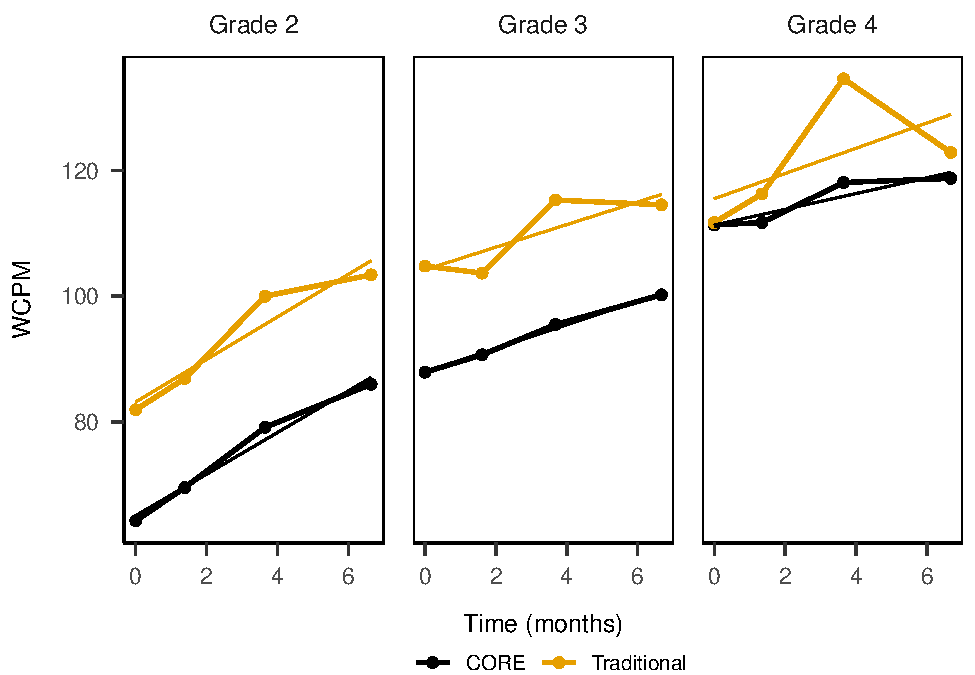
\includegraphics{conseq_validity_manusript_files/figure-latex/fig-means-1.pdf}
\caption{\label{fig:fig-means}Mean words correct per minute (WCPM) score across waves by grade and CBM-R measure.}
\end{figure}

Table~\ref{tab:tbl-desc} shows the descriptive WCPM data, and Figure~\ref{fig:fig-means} shows the WCPM means for each wave.

\hypertarget{core-cbm-r}{%
\subsubsection{CORE CBM-R}\label{core-cbm-r}}

Each CORE passage is an original work of narrative fiction that follows the story grammar of English language short stories, with a main character and a clear beginning, middle, and end (link blinded for review). To reduce construct-irrelevant variance associated with different authors' voice and style, the author of the CORE passages was part of the team that authored the easyCBM traditional CBM-R passages used in this study. Apart from the passage length requirements, the CORE passages were written to similar specifications as the easyCBM passages. Each CORE passage was written within 5 words of a targeted length: long = 85 words or medium = 50 words. Ultimately, 150 passages were written: 50 at each of Grades 2-4, with 20 long passages and 30 medium passages for each grade.

Administration instructions were to allow students to read the CORE passages in their entirety, but a time limit was set at 90 s. At each wave, sample students read on average 8.40 passages (\emph{SD} = 1.80; range = 1 - 12).

The CORE scores are model-based estimates of WCPM, based on a recently proposed latent-variable psychometric model of speed and accuracy for CBM-R data (Kara, Kamata, Potgieter, \& Nese, 2020). The model-based CBM-R WCPM estimates are based on a two-part model that includes components for reading accuracy and reading speed. The accuracy component is a binomial-count factor model, where accuracy is measured by the number of correctly read words in the passage. The speed component is a log-normal factor model, where speed is measured by passage reading time. Parameters in the accuracy and speed models are jointly modeled and estimated. For a detailed description, please see Kara et al. (2020).

\hypertarget{traditional-cbm-r}{%
\subsubsection{Traditional CBM-R}\label{traditional-cbm-r}}

We administered the easyCBM (Alonzo, Tindal, Ulmer, \& Glasgow, 2006) oral reading fluency measures as the traditional CBM-R assessments for the purpose of comparison to CORE passages. easyCBM CBM-R passages range from 200 to 300 words in length and are original works of fiction developed to be of equivalent difficulty for each grade level following word-count, grade-level guidelines (e.g., Flesch-Kincaid readability estimates), and form equivalence empirical testing using repeated measures ANOVA to evaluate comparability of forms (Alonzo \& Tindal, 2007). The easyCBM CBM-R measures have demonstrated features of technical adequacy that suggest they are sufficient to meet the needs as the comparative example of an existing traditional CBM-R assessment (Anderson et al., 2014). The reported alternate form reliability across passages ranged from .83 to .98, test-retest reliability ranged from .84 to .96, and G-coefficients ranged from .94 to .98 (Anderson et al., 2014). Predictive (fall, winter) and concurrent (spring) relations between Grade 2 CBM-R and spring SAT-10 reading scale scores were .59 to .62, and .66 respectively (Anderson et al., 2014).

Following standard administration protocols, students were given 60 s to read the traditional CBM-R passages.

\hypertarget{asr-scoring}{%
\paragraph{ASR Scoring}\label{asr-scoring}}

The ASR engine scored each audio recording file, scoring each word as read correctly or incorrectly, and recording the time in centi-seconds to read each word and the time between words. Bavieca, an open-source speech recognition toolkit, was the ASR applied in this study (\url{http://www.bavieca.org/}). Bavieca uses continuous density hidden Markov models and supports maximum likelihood linear regression, vocal tract length normalization, and discriminative training (maximum mutual information). It uses the general approach of many state-of-the art speech recognition systems: a Viterbi Beam Search used to find the optimal mapping of the speech input onto a sequence of words. The score for a word sequence was calculated by interpolating language model scores and acoustic model scores. The language model assigned probabilities to sequences of words using trigrams (where the probability of the next word is conditioned on the two previous words) and was trained using the CMU-Cambridge LM Toolkit (Clarkson \& Rosenfeld, 1997). Acoustic models were clustered triphones based on Hidden Markov Models using Gaussian Mixtures to estimate the probabilities of the acoustic observation vectors. The system used filler models to match the types of disfluencies found in applications.

\hypertarget{cbm-comprehension}{%
\subsubsection{CBM Comprehension}\label{cbm-comprehension}}

The easyCBM comprehension measure assesses students' comprehension of a 1,500 word fictional narrative. The comprehension items are designed to target students' literal (7 items), inferential (7 items), and evaluative (6 items) comprehension. Split-half reliability ranged from .38 to .87, item reliability from Rasch analyses ranged from .39 to .94, and Cronbach's alpha ranged from .69 to .78 (Saez et al., 2010). Predictive (fall) and concurrent (spring) correlations between Grade 2 CBM comprehension and spring SAT-10 reading scale scores were .62 and .66 respectively (Jamgochian et al., 2010). Predictive (fall) and concurrent (spring) correlations between Grade 3 and 4 CBM comprehension and spring state reading test scores (Oregon Assessment of Knowledge and Skills {[}OAKS{]} and Washington Measures of Student Progress {[}MSP{]}) were .52 to .70, and .37 to .68 respectively (Anderson et al., 2014). Predictive diagnostic statistics for fall CBM comprehension and spring state reading test scores included sensitivity from .68 to .86, specificity from .57 to .92, and AUC from .74 to .86. Concurrent diagnostic statistics for spring CBM comprehension and spring state reading test scores included sensitivity from .69 to .89, specificity from .63 to .80, and AUC ranged from .76 to .87 (Anderson et al., 2014).

The Grade 2 CBM Comprehension measure contains 12 multiple-choice items (Mean = 10.40, \emph{SD} = 1.70), whereas the Grade 3 (Mean = 14.10, \emph{SD} = 4.10) and Grade 4 (Mean = 13.50, \emph{SD} = 3.80) measures contain 20 multiple-choice items.

Figure~\ref{fig-comp-scatter} shows scatter plots of the CBM-R WCPM and CBM Comprehension scores by grade and season (distal and proximal).



\begin{figure}
\centering
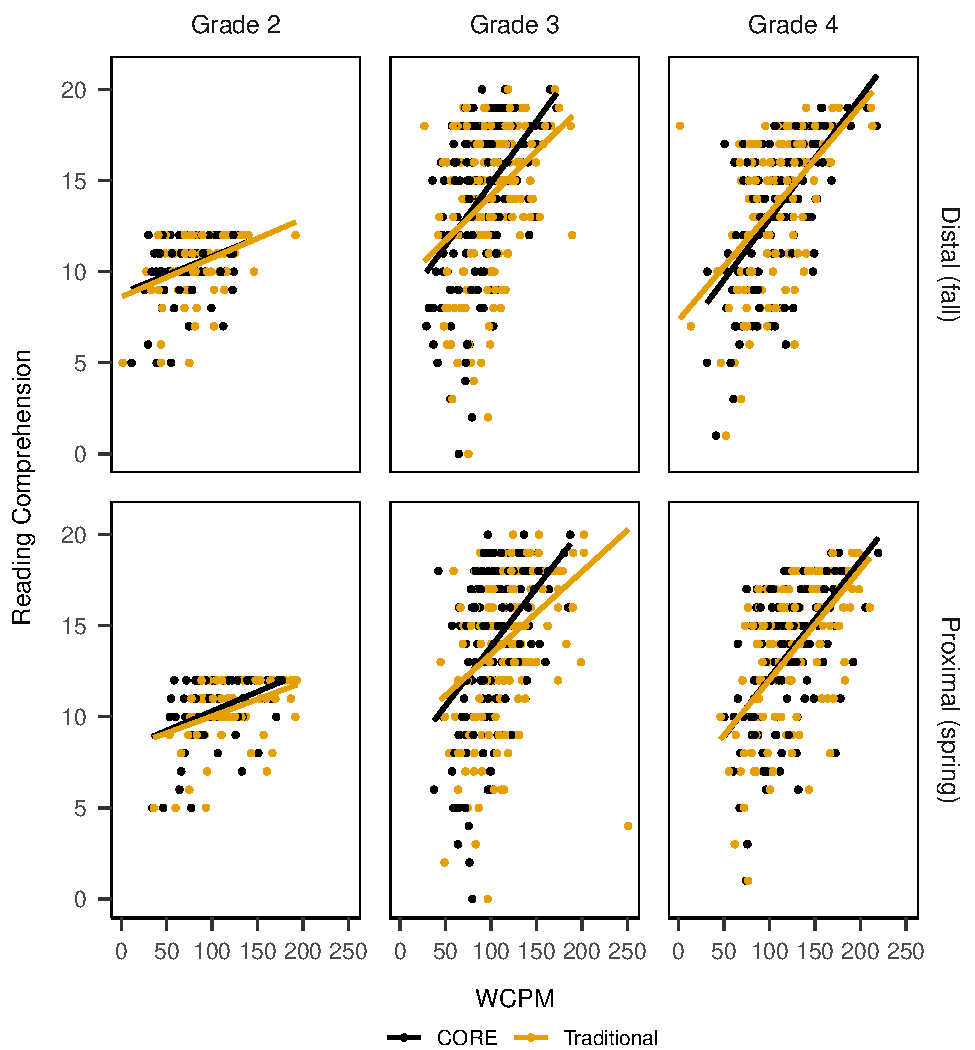
\includegraphics{conseq_validity_manusript_files/figure-latex/fig-comp-scatter-1.pdf}
\caption{\label{fig:fig-comp-scatter}Words correct per minute (WCPM) and CBM Comprehension scores by grade and season, distal (fall) and proximal (spring).}
\end{figure}

\hypertarget{sbac-reading-test}{%
\subsubsection{SBAC Reading Test}\label{sbac-reading-test}}

The Smarter Balanced Assessment Consortium (SBAC) English language arts/literacy (ELA/L) summative assessment is administered to students in Grades 3 through 8 and 11 and consists of two parts: a computerized adaptive test (CAT), and a performance task (PT) component. The SBAC ELA/L was developed to align to the Common Core State Standards (CCSS) and measures four broad clams: reading, writing, listening, and research (Consortium, 2020). Within each claim there are a number of assessment targets, and each test item is aligned to a specific claim and target and to a CCSS (CITE). The CAT consisted of selected response items that assess all four claims. The PT consisted of a set of related stimuli presented with two or three research items requiring both short-text responses and a full written response that assess the writing and research claims. The overall SBAC ELA/L performance scaled score is divided into four proficiency categories, Well Below, Below, Proficient, and Advanced, where the third and fourth categories designate meeting grade-level achievement standards.

The mean SBAC ELA/L score for Grade 3 was 2,446.90 (\emph{SD} = 74.80) with 61\% meeting proficiency. The mean SBAC ELA/L score for Grade 4 was 2480 (\emph{SD} = 79.70) with 57 `\% meeting proficiency.

Figure~\ref{fig-sbac-scatter} shows scatter and density plots of the CBM-R WCPM and SBAC ELA/L score and proficiency, respectively, by grade and season (distal and proximal).



\begin{figure}
\centering
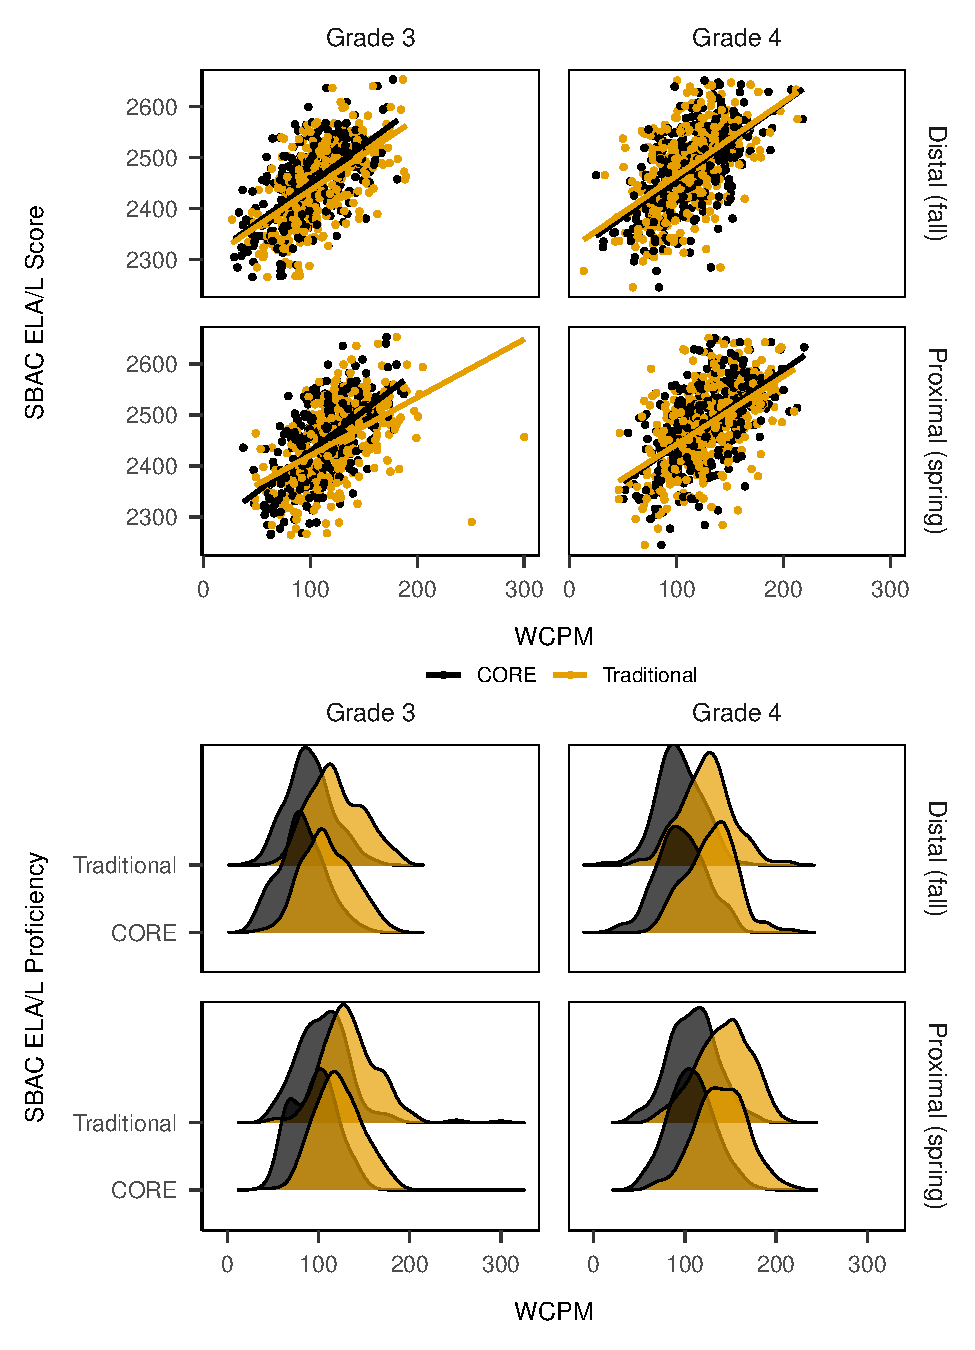
\includegraphics{conseq_validity_manusript_files/figure-latex/fig-sbac-scatter-1.pdf}
\caption{\label{fig:fig-sbac-scatter}Words correct per minute (WCPM) and SBAC ELA/L Score \& Proficiency classification by grade and season, distal (fall) and proximal (spring).}
\end{figure}

\hypertarget{procedure}{%
\subsection{Procedure}\label{procedure}}

Students were assessed online, using classroom or school devices, and wore headphones with an attached noise-cancelling microphone provided by the research team. Students were given a task introduction by their teacher, and then directed to the study website where the first page asked for student assent (if a student declined, their participation ended). The standardized instructions were presented via audio as well as print. \emph{\enquote{Get ready! You are about to do some reading! After pressing start, read the story on the screen. When you are finished click done. Do your best reading, and have fun!}}

For each of the four measurement occasions (Oct-Nov 2017, 2018; Nov-Feb 2017-18, 2018-19; Feb-Mar 2018, 2019; May-Jun, 2018, 2019), students read aloud online a randomly assigned, fixed set of 10 to 12 CORE passages (3-5 long and 5-7 medium), and one traditional CBM-R passage from the easyCBM progress monitoring system.

An automatic speech recognition engine scored each reading, scoring each word as read correctly or incorrectly (accuracy), and recording the time duration to read each word (and the silence between) which was aggregated to calculate the time to read the passage (speed).

All WCPM scores were based on these readings and data. The model-based WCPM CORE scores (Kara et al., 2020) were estimated for each measurement occasion based on the number CORE passages read. Traditional CBM-R WCPM scores were calculated by dividing the number of words read correctly (wrc) by the quotient of the total seconds read (sec) and 60 (i.e., \(wrc/(sec/60)\)).

\hypertarget{analyses}{%
\subsection{Analyses}\label{analyses}}

To address RQ 1, we applied a latent growth model (LGM; Meredith and Tisak (1990)) separately for each grade to represent students' within-year oral reading fluency growth. The linear time covariate was specified as the elapsed number of months between the median month at wave \(t\) and the median month of \(t_1\) (see Table~\ref{tab:tbl-desc}).

Two results are extracted from the LGMs to compare the growth properties of the traditional CBM-R and model-based CORE scores. One, the fixed intercept and slope estimates and their associated standard errors (\emph{SE}), as estimated by the linear growth model. Two, the reliability of the CBM-R scores at each wave, as estimated by the proportion of true score variance to observed score variance (Rogosa \& Willett, 1983; Singer, Willett, Willett, \& others, 2003; Willett, 1988). EDIT

\[
\rho_t = \frac{\psi_{00} + \lambda^2_t \psi_{11} + 2\lambda_t \psi_{01}}{\psi_{00} + \lambda^2_t \psi_{11} + 2\lambda_t \psi_{01} + \theta_t} = \frac{var(y_t) - \theta_t}{var(y_t)} 
\]
Where \(\rho_t\) represent the reliability at wave \(t\), \(\psi\) represents the covariance structure of the intercept and slope factors, \(\lambda_t\) represents the linear time covariate, and \(\theta_t\) represents the residual variance at a wave, which is equivalent to the ratio of the true score variance (\(var(y_t) - \theta_t\)) to the observed score variance (\(var(y_t)\)), and can be calculated for each wave by subtracting the residual variance (measurement error) from the observed score variance. This estimate of reliability provides both the true score variance explained by the longitudinal model and the unique measurement error variance of observed scores at each wave, and has been applied for estimating reliability of CBM data (Yeo, Kim, Branum-Martin, Wayman, \& Espin, 2012).

All analyses and figures were conducted and created in the R programming environment (R Core Team, 2020). The LGM analyses were conducted using the lavaan package with maximum likelihood estimation with robust (Huber-White) standard errors and a scaled test statistic that is (asymptotically) equal to the Yuan-Bentler test statistic (Rosseel, 2012). This estimator is robust to non-normality and clustering (McNeish, Stapleton, \& Silverman, 2017).

To address RQs 2 and 3, we apply a predictive approach to determine which CBM-R predictor most accurately estimates the outcomes, rather an inferential approach that pursues unbiased estimates of \(\beta\) coefficients. Our predictive model is a linear model, separate for by grade and CBM-R predictor, regressing the outcome (spring CBM comprehension, SBAC ELA/L scores, or SBAC ELA/L proficiency) on the CBM-R predictor (traditional CBM-R scores vs.~CORE model-based scores from fall or spring).

For RQ 2, we fit 12 linear models: 2 CBM-R predictors each at 2 seasons (fall and spring) for each of 3 grades: \(Comprehension_i = \beta_0 + \beta_1CBM\mbox{-}R_{season} + \epsilon_i\).

For RQ 3, we model Grades 3 and 4 together and thus include grade level as a categorical covariate, as well as the state (to account for differences in standards). We fit 8 linear models, applying a logistic regression for the categorical SBAC ELA/L proficiency outcome: \(SBAC_i = \beta_0 + \beta_1CBM\mbox{-}R_{season} + Grade + State + \epsilon_i\).

To measure the accuracy of the models, our predictive performance measures were the \emph{RMSEA} and \(R^2\) for the continuous outcomes (spring CBM comprehension and SBAC ELA/L scores), and the Receiver Operating Characteristic (ROC) area under the curve (AUC) for the categorical outcome (SBAC ELA/L proficiency).

To understand the predictive accuracy of the CBM-R measures, and how their accuracy might generalize to new data, we split the data (by RQ) into two sets: a training set, a random sample of 75\% of the data; and a test set, the remaining 25\% of the data.

To get a measure of variance for the performance measures, we apply 10 fold cross-validation to the training set. For each fold, 10\% of the training set is sampled and serves as an assessment sample, so that each observation serves in one and only one assessment sample. The remaining 90\% of the training set serve as the analysis sample for a fold. The predictive model (Eq 2) is fit on the 90\% analysis sample of each fold, and the resulting model parameters are used to predict the assessment sample within each fold. The performance measures (\emph{RMSEA} and AUC) are taken from each fold, and the final performance is the mean performance measure across the 10 folds, and the of variance around the mean.

Research has shown that 10 folds is a sensible value for \emph{k}-fold cross-validation, and repeating \emph{k}-fold cross-validation can improve the accuracy of the estimates while maintaining small bias, particularly for smaller sample sizes (Kim, 2009; Molinaro, Simon, \& Pfeiffer, 2005). We apply 10-fold cross-validation repeated 5 times for each RQ so that we fit 50 models and record 50 performance measures to the training set (10 folds \(\times\) 5 repeats = 50).

Finally, we fit the predictive models to the entire training set, and then use the resulting model parameters to predict the results of the test set. The test set here can be can be conceptualized as \enquote{new} (or unseen) data, as it has not been used to this point. The resulting final performance measures serve as estimates of how the two comparison CBM-R measures will generalize in their predictive accuracy.

The predictive modeling process was conducted using the tidymodels package (Kuhn \& Wickham, 2020). We also used the following R packages: doParallel (Corporation \& Weston, 2020), ggridges(Wilke, 2020), ggthemes (Arnold, 2019), gt (Iannone, Cheng, \& Schloerke, 2020), janitor (Firke, 2020), lavaan (Rosseel, 2012), papaja (Aust \& Barth, 2020), patchwork (Pedersen, 2020), tidyverse (Wickham et al., 2019).

\hypertarget{results}{%
\section{Results}\label{results}}

\hypertarget{rq1}{%
\subsubsection{RQ1}\label{rq1}}

To address RQ 1, we fit LGMs separately for each CBM-R measure and grade.

\captionsetup[table]{labelformat=empty,skip=1pt}
\begin{longtable}{lllllll}
\caption*{
\large Table 3.<br><br><i>Latent Growth Model Parameter Estimates by Grade </i>\\ 
} \\ 
\toprule
& \multicolumn{3}{c}{CORE} & \multicolumn{3}{c}{Traditional} \\ 
 \cmidrule(lr){2-4}\cmidrule(lr){5-7}
 & Parameter & \emph{SE} & \emph{z}-value & Parameter & \emph{SE} & \emph{z}-value \\ 
\midrule
\multicolumn{1}{l}{Grade 2} \\ 
\midrule
Mean Intercept & 63.75 & 1.39 & 45.86 & 74.79 & 1.31 & 56.89 \\ 
Mean Slope & 3.59 & 0.13 & 27.40 & 4.30 & 0.21 & 20.55 \\ 
Variance Intercept & 1070.46 & 56.82 & 18.84 & 694.73 & 54.94 & 12.65 \\ 
Variance Slope & 3.04 & 1.03 & 2.95 & 5.25 & 2.06 & 2.55 \\ 
Correlation Intercept-Slope & -0.35 & -- & -- & 0.05 & -- & -- \\ 
Residual Variance Wave 1 & 108.15 & 21.60 & 5.01 & 174.89 & 39.26 & 4.46 \\ 
Residual Variance Wave 2 & 123.28 & 30.80 & 4.00 & 170.13 & 21.54 & 7.90 \\ 
Residual Variance Wave 3 & 188.05 & 33.71 & 5.58 & 383.15 & 108.25 & 3.54 \\ 
Residual Variance Wave 4 & 166.29 & 43.15 & 3.85 & 164.71 & 56.55 & 2.91 \\ 
\midrule
\multicolumn{1}{l}{Grade 3} \\ 
\midrule
Mean Intercept & 86.86 & 1.27 & 68.56 & 98.34 & 1.25 & 78.41 \\ 
Mean Slope & 2.00 & 0.11 & 17.69 & 2.33 & 0.15 & 15.06 \\ 
Variance Intercept & 1154.59 & 61.11 & 18.89 & 861.74 & 72.83 & 11.83 \\ 
Variance Slope & 2.96 & 1.20 & 2.46 & 0.87 & 2.57 & 0.34 \\ 
Correlation Intercept-Slope & -0.51 & -- & -- & 0.25 & -- & -- \\ 
Residual Variance Wave 1 & 86.29 & 17.68 & 4.88 & 211.07 & 57.28 & 3.68 \\ 
Residual Variance Wave 2 & 170.98 & 22.35 & 7.65 & 345.25 & 88.15 & 3.92 \\ 
Residual Variance Wave 3 & 175.85 & 25.57 & 6.88 & 325.07 & 42.81 & 7.59 \\ 
Residual Variance Wave 4 & 173.13 & 35.41 & 4.89 & 245.04 & 75.52 & 3.24 \\ 
\midrule
\multicolumn{1}{l}{Grade 4} \\ 
\midrule
Mean Intercept & 109.71 & 1.30 & 84.62 & -- & -- & -- \\ 
Mean Slope & 1.67 & 0.11 & 15.06 & -- & -- & -- \\ 
Variance Intercept & 1125.18 & 63.04 & 17.85 & -- & -- & -- \\ 
Variance Slope & 0.74 & 1.15 & 0.64 & -- & -- & -- \\ 
Correlation Intercept-Slope & -0.44 & -- & -- & -- & -- & -- \\ 
Residual Variance Wave 1 & 103.88 & 20.96 & 4.96 & -- & -- & -- \\ 
Residual Variance Wave 2 & 167.61 & 33.84 & 4.95 & -- & -- & -- \\ 
Residual Variance Wave 3 & 149.52 & 21.61 & 6.92 & -- & -- & -- \\ 
Residual Variance Wave 4 & 207.36 & 46.01 & 4.51 & -- & -- & -- \\ 
\bottomrule
\end{longtable}

The fit measures for the Grade 2 CORE LGM were \(\chi^2\) = 13.70 with \emph{df} = 5 (\emph{p} = .018), Tucker--Lewis fit (TLI) = 1, Comparative Fit Index (CFI) = 1, \emph{RMSEA} = 0.04, and BIC = 17,986.3. The fit measures for the Grade 2 Traditional LGM were \(\chi^2\) = 56.40 with \emph{df} = 5 (\emph{p} \textless{} .001), TLI = 0.93, CFI = 0.94, \emph{RMSEA} = 0.13, and BIC = 13,647.1. The fit measures for the Grade 3 CORE LGM were \(\chi^2\) = 9.20 with \emph{df} = 5 (\emph{p} = .100), TLI = 1, CFI = 1, \emph{RMSEA} = 0.03, and BIC = 23,365.1. The fit measures for the Grade 3 Traditional LGM were \(\chi^2\) = 65.10 with \emph{df} = 5 (\emph{p} \textless{} .001), TLI = 0.96, CFI = 0.96, \emph{RMSEA} = 0.11, and BIC = 19,956.8. The fit measures for the Grade 4 CORE LGM were \(\chi^2\) = 28.50 with \emph{df} = 5 (\emph{p} \textless{} .001), TLI = 0.99, CFI = 0.99, \emph{RMSEA} = 0.08, and BIC = 21,461.1)`.

The Grade 4 LGM for Traditional CBM-R was not successfully estimated without a negative variance for the slope factor. We tried alternate modeling solutions, including homogeneous residual variances (and zero error covariances), heterogeneous Teoplitz residual structure, first-order autocorrelated residuals (McNeish \& Harring, 2019), and transformed slope factor loadings, but all models were unsuccessful due to a negative variance or variance-covariance matrix. Thus, we do not report the results from this model.

Table~\ref{tab:tbl-lgms-results} shows the parameter estimates from the LGMs. The \emph{SE} for the mean intercept estimates across grades are slightly larger for the model-based CORE models (1.27 to 1.39) than the traditional CBM-R models (1.25 to 1.31); however, the \emph{SE} for the mean slope estimates for the model-based CORE models (0.11 to 0.13) are about a third of the size as those of the traditional CBM-R models (0.15 to 0.21).

Table~\ref{tab:tbl-lgms-reliab} shows the observed variances CBM-Rs at each wave, the estimated residual variances from the LGMs, and reliability estimates by grade and wave. Across grades and waves, the reliability estimates were higher for the model-based CORE scores except for Grade 2, wave 4 (.85 vs.~.86). The reliability estimates for the model-based CORE scores ranged from .82 to .93, and for the Traditional CBM-R ranged from .62 to .86.

\hypertarget{rq2}{%
\subsection{RQ2}\label{rq2}}

To address RQ 2 we used a predictive approach with resampling and fit linear models separate for by grade and CBM-R predictor, regressing the spring CBM comprehension on the CBM-R predictors.

\begin{verbatim}
## 69.47 sec elapsed
\end{verbatim}

\captionsetup[table]{labelformat=empty,skip=1pt}
\begin{longtable}{rrrrrrrrrrrrr}
\caption*{
\large Table 5.<br><br><i>Spring CBM Comprehension Predictive Measures (RMSE and R<sup>2</sup>) For Distal and Proximal CBM-R Predictors by Grade</i>\\ 
} \\ 
\toprule
& \multicolumn{6}{c}{CORE} & \multicolumn{6}{c}{Traditional} \\ 
 \cmidrule(lr){2-7}\cmidrule(lr){8-13}
 & Mean \emph{RMSE} & \emph{SE} & Mean <em>R</em><sup>2</sup> & \emph{SE} & \textbf{Final \emph{RMSE}} & <b>Final <em>R</em><sup>2</sup></b> & Mean \emph{RMSE} & \emph{SE} & Mean <em>R</em><sup>2</sup> & \emph{SE} & \textbf{Final \emph{RMSE}} & <b>Final <em>R</em><sup>2</sup></b> \\ 
\midrule
\multicolumn{1}{l}{Distal} \\ 
\midrule
Grade 2 & 1.41 & (0.07) & 0.21 & (0.03) & 1.96 & 0.36 & 1.42 & (0.07) & 0.23 & (0.03) & 1.90 & 0.34 \\ 
Grade 3 & 3.46 & (0.09) & 0.24 & (0.02) & 3.96 & 0.24 & 3.66 & (0.10) & 0.17 & (0.02) & 4.22 & 0.13 \\ 
Grade 4 & 3.06 & (0.08) & 0.38 & (0.03) & 2.73 & 0.48 & 3.34 & (0.11) & 0.31 & (0.03) & 2.84 & 0.44 \\ 
\midrule
\multicolumn{1}{l}{Proximal} \\ 
\midrule
Grade 2 & 1.41 & (0.07) & 0.25 & (0.03) & 1.89 & 0.49 & 1.38 & (0.07) & 0.27 & (0.03) & 1.92 & 0.33 \\ 
Grade 3 & 3.49 & (0.08) & 0.23 & (0.02) & 4.08 & 0.20 & 3.64 & (0.13) & 0.24 & (0.02) & 4.21 & 0.14 \\ 
Grade 4 & 3.21 & (0.10) & 0.34 & (0.03) & 2.71 & 0.48 & 3.17 & (0.10) & 0.37 & (0.03) & 2.83 & 0.39 \\ 
\bottomrule
\end{longtable}

For RQ 2 we compared the predictive accuracy of traditional CBM-R and CORE for distal (fall) and proximal (spring) assessments predicting spring CBM comprehension scores for students in Grades 2 through 4. Table~\ref{tab:tbl-pred-comp} shows the mean \emph{RMSE} and \(R^2\) values across the 50 models fit the 10-fold cross-validation samples, as well as the final \emph{RMSE} and \(R^2\) values for the train/test sample. For the distal (fall) CBM-R predictors, the results generally favor CORE, which has better (lower) mean \emph{RMSE} values across grades compared to Traditional CBM-R, and better (higher) mean \(R^2\) values for Grades 3 and 4 (but not Grade 2). For the proximal (spring) CBM-R predictors, the results generally favor traditional CBM-R, which has lower \emph{RMSE} values for Grades 2 and 4 (but not Grade 3), and higher \(R^2\) values across grades. To give context to the \emph{RMSE} values, note that the CBM Comprehension assessment has 12 items for Grade 2 and 20 items for Grades 3 and 4, with \emph{SD}s of 1.69, 4.06, and 3.80, respectively, so the \emph{RMSE} values are generally smaller than the sample \emph{SD}s.

The final \emph{RMSE} and \(R^2\) values in Table~\ref{tab:tbl-pred-comp} represent the parameters of the predictive models applied to the training set (75\% of sample) used to predict the test set (25\% of sample). For both the distal (fall) and proximal (spring) CBM-R predictors, the results favor CORE, which had lower \emph{RMSE} and higher \(R^2\) values across all comparisons (except Grade 2, distal \emph{RMSE}). The \emph{RMSE} values represent differences of 2\% to 7\% of a \emph{SD} favoring CORE, and 4\% of a \emph{SD} favoring Traditional CBM-R for the Grade 2 distal model. The \(R^2\) values represent increases in explained variance for CORE above Traditional CBM-R of 5\% to 82\%.

\hypertarget{rq3}{%
\subsection{RQ3}\label{rq3}}

To address RQ 3 we used again used a predictive approach with resampling and fit linear models separate for by grade and CBM-R predictor, regressing SBAC ELA/L (score or proficiency) on the CBM-R predictors, grade, and state.

\begin{verbatim}
## 67.31 sec elapsed
\end{verbatim}

\captionsetup[table]{labelformat=empty,skip=1pt}
\begin{longtable}{lll}
\caption*{
\large Table 6.<br><br><i>SBAC ELA/L Predictive Measures (RMSE and R<sup>2</sup>) For Distal and Proximal CBM-R Predictors by Grade</i>\\ 
} \\ 
\toprule
 & CORE & Traditional \\ 
\midrule
\multicolumn{1}{l}{Distal - SBAC Score} \\ 
\midrule
Mean \emph{RMSE} (\emph{SE}) & 60.19 (0.70) & 60.54 (0.64) \\ 
Mean \emph{R}2 (\emph{SE}) & 0.40 (0.01) & 0.40 (0.01) \\ 
\textbf{Final \emph{RMSE}} & 62.60  & 68.03  \\ 
\textbf{Final \emph{R}2} & 0.42  & 0.31  \\ 
\midrule
\multicolumn{1}{l}{Proximal - SBAC Score} \\ 
\midrule
Mean \emph{RMSE} (\emph{SE}) & 60.56 (0.69) & 64.14 (0.96) \\ 
Mean \emph{R}2 (\emph{SE}) & 0.40 (0.01) & 0.34 (0.02) \\ 
\textbf{Final \emph{RMSE}} & 62.44  & 66.70  \\ 
\textbf{Final \emph{R}2} & 0.42  & 0.34  \\ 
\midrule
\multicolumn{1}{l}{Distal - SBAC Proficiency} \\ 
\midrule
Mean Accuracy (\emph{SE}) & 0.73 (0.01) & 0.72 (0.01) \\ 
Mean AUC (\emph{SE}) & 0.80 (0.01) & 0.79 (0.01) \\ 
\textbf{Final Accuracy} & 0.73  & 0.68  \\ 
\textbf{Final AUC} & 0.79  & 0.75  \\ 
\midrule
\multicolumn{1}{l}{Proximal - SBAC Proficiency} \\ 
\midrule
Mean Accuracy (\emph{SE}) & 0.74 (0.01) & 0.74 (0.01) \\ 
Mean AUC (\emph{SE}) & 0.80 (0.01) & 0.80 (0.01) \\ 
\textbf{Final Accuracy} & 0.73  & 0.69  \\ 
\textbf{Final AUC} & 0.80  & 0.78  \\ 
\bottomrule
\end{longtable}

For RQ 3 we compared the predictive accuracy of traditional CBM-R and CORE for distal (fall) and proximal (spring) assessments predicting spring SBAC ELA/L (scores and profiency classification) for students in Grades 3 and 4.

Table~\ref{tab:tbl-pred-sbac} shows the mean \emph{RMSE} and \(R^2\) values across the 50 models fit the 10-fold cross-validation samples, as well as the final \emph{RMSE} and \(R^2\) values for the train/test sample. For the SBAC ELA/L score (continuous) outcome, the distal results favored CORE which had lower mean and final \emph{RMSE} and higher mean and final \(R^2\) values across grades compared to Traditional CBM-R. To give context to the \emph{RMSE} values, the \emph{SD} of SBAC ELA/L was 79 for Grades 3 and 4 combined, so the \emph{RMSE} values were approximately three-quarters of a \emph{SD}.

For the SBAC ELA/L proficiency (classification) outcome with distal predictors, CORE had higher Accuracy and AUC values across grades compared to Traditional CBM-R. For the proximal predictors, the results were generally comparable. CORE had a slightly higher Mean AUC (0.80 vs.~0.78), Traditional CBM-R had a slightly higher final accuracy (0.69 vs.~0.73), and they had the equivalent Mean Accuracy and Final AUC values.

\hypertarget{discussion}{%
\section{Discussion}\label{discussion}}

THESE REPRESENT THE VALUES EXPECTED IN A NEW SAMPLE\ldots These final performance measures serve as estimates of how the two comparison CBM-R measures may generalize in their predictive accuracy.

\newpage

\hypertarget{references}{%
\section{References}\label{references}}

\begingroup
\setlength{\parindent}{-0.5in}
\setlength{\leftskip}{0.5in}

\hypertarget{refs}{}
\leavevmode\hypertarget{ref-alonzotindal2007}{}%
Alonzo, J., \& Tindal, G. (2007). The development of word and passage reading fluency measures for use in a progress monitoring assessment system. Technical report\# 40. \emph{Behavioral Research and Teaching}.

\leavevmode\hypertarget{ref-anderson2014tech}{}%
Anderson, D., Alonzo, J., Tindal, G., Farley, D., Irvin, P. S., Lai, C.-F., \ldots{} Wray, K. A. (2014). Technical manual: EasyCBM. Technical report\# 1408. \emph{Behavioral Research and Teaching}.

\leavevmode\hypertarget{ref-ggthemes}{}%
Arnold, J. B. (2019). \emph{Ggthemes: Extra themes, scales and geoms for 'ggplot2'}. Retrieved from \url{https://CRAN.R-project.org/package=ggthemes}

\leavevmode\hypertarget{ref-papaja}{}%
Aust, F., \& Barth, M. (2020). \emph{papaja: Create APA manuscripts with R Markdown}. Retrieved from \url{https://github.com/crsh/papaja}

\leavevmode\hypertarget{ref-sbac}{}%
Consortium, S. B. A. (2020). Smarter balanced 2018-19 summative technical report. Retrieved February 24, 2021, from \url{https://technicalreports.smarterbalanced.org/2018-19_summative-report/_book/index.html}

\leavevmode\hypertarget{ref-doParallel}{}%
Corporation, M., \& Weston, S. (2020). \emph{DoParallel: Foreach parallel adaptor for the 'parallel' package}. Retrieved from \url{https://CRAN.R-project.org/package=doParallel}

\leavevmode\hypertarget{ref-janitor}{}%
Firke, S. (2020). \emph{Janitor: Simple tools for examining and cleaning dirty data}. Retrieved from \url{https://CRAN.R-project.org/package=janitor}

\leavevmode\hypertarget{ref-gt}{}%
Iannone, R., Cheng, J., \& Schloerke, B. (2020). \emph{Gt: Easily create presentation-ready display tables}. Retrieved from \url{https://github.com/rstudio/gt}

\leavevmode\hypertarget{ref-jamgochian2010tech}{}%
Jamgochian, E., Park, B. J., Nese, J. F., Lai, C.-F., Sáez, L., Anderson, D., \ldots{} Tindal, G. (2010). Technical adequacy of the easyCBM grade 2 reading measures. Technical report\# 1004. \emph{Behavioral Research and Teaching}.

\leavevmode\hypertarget{ref-kara2020}{}%
Kara, Y., Kamata, A., Potgieter, C., \& Nese, J. F. (2020). Estimating model-based oral reading fluency: A bayesian approach. \emph{Educational and Psychological Measurement}, \emph{80}(5), 847--869.

\leavevmode\hypertarget{ref-kim2009}{}%
Kim, J.-H. (2009). Estimating classification error rate: Repeated cross-validation, repeated hold-out and bootstrap. \emph{Computational Statistics \& Data Analysis}, \emph{53}(11), 3735--3745.

\leavevmode\hypertarget{ref-tidymodels}{}%
Kuhn, M., \& Wickham, H. (2020). \emph{Tidymodels: A collection of packages for modeling and machine learning using tidyverse principles.} Retrieved from \url{https://www.tidymodels.org}

\leavevmode\hypertarget{ref-mcneish2019}{}%
McNeish, D., \& Harring, J. (2019). Covariance pattern mixture models: Eliminating random effects to improve convergence and performance. \emph{Behavior Research Methods}, 1--33.

\leavevmode\hypertarget{ref-mcneishetal2017}{}%
McNeish, D., Stapleton, L. M., \& Silverman, R. D. (2017). On the unnecessary ubiquity of hierarchical linear modeling. \emph{Psychological Methods}, \emph{22}(1), 114.

\leavevmode\hypertarget{ref-meredithtisak1990}{}%
Meredith, W., \& Tisak, J. (1990). Latent curve analysis. \emph{Psychometrika}, \emph{55}(1), 107--122.

\leavevmode\hypertarget{ref-molinaro2005}{}%
Molinaro, A. M., Simon, R., \& Pfeiffer, R. M. (2005). Prediction error estimation: A comparison of resampling methods. \emph{Bioinformatics}, \emph{21}(15), 3301--3307.

\leavevmode\hypertarget{ref-patchwork}{}%
Pedersen, T. L. (2020). \emph{Patchwork: The composer of plots}. Retrieved from \url{https://CRAN.R-project.org/package=patchwork}

\leavevmode\hypertarget{ref-R-base}{}%
R Core Team. (2020). \emph{R: A language and environment for statistical computing}. Vienna, Austria: R Foundation for Statistical Computing. Retrieved from \url{https://www.R-project.org/}

\leavevmode\hypertarget{ref-rogosaetal1983}{}%
Rogosa, D. R., \& Willett, J. B. (1983). Demonstrating the reliability of the difference score in the measurement of change. \emph{Journal of Educational Measurement}, 335--343.

\leavevmode\hypertarget{ref-lavaan}{}%
Rosseel, Y. (2012). lavaan: An R package for structural equation modeling. \emph{Journal of Statistical Software}, \emph{48}(2), 1--36. Retrieved from \url{http://www.jstatsoft.org/v48/i02/}

\leavevmode\hypertarget{ref-saez2010tech}{}%
Saez, L., Park, B., Nese, J. F., Jamgochian, E., Lai, C.-F., Anderson, D., \ldots{} Tindal, G. (2010). Technical adequacy of the easyCBM reading measures (grades 3-7), 2009-2010 version. Technical report\# 1005. \emph{Behavioral Research and Teaching}.

\leavevmode\hypertarget{ref-singerwillett2003}{}%
Singer, J. D., Willett, J. B., Willett, J. B., \& others. (2003). \emph{Applied longitudinal data analysis: Modeling change and event occurrence}. Oxford university press.

\leavevmode\hypertarget{ref-tidyverse}{}%
Wickham, H., Averick, M., Bryan, J., Chang, W., McGowan, L. D., François, R., \ldots{} Yutani, H. (2019). Welcome to the tidyverse. \emph{Journal of Open Source Software}, \emph{4}(43), 1686. \url{https://doi.org/10.21105/joss.01686}

\leavevmode\hypertarget{ref-ggridges}{}%
Wilke, C. O. (2020). \emph{Ggridges: Ridgeline plots in 'ggplot2'}. Retrieved from \url{https://CRAN.R-project.org/package=ggridges}

\leavevmode\hypertarget{ref-willett1988chapter}{}%
Willett, J. B. (1988). Chapter 9: Questions and answers in the measurement of change. \emph{Review of Research in Education}, \emph{15}(1), 345--422.

\leavevmode\hypertarget{ref-yeoetal2012}{}%
Yeo, S., Kim, D.-I., Branum-Martin, L., Wayman, M. M., \& Espin, C. A. (2012). Assessing the reliability of curriculum-based measurement: An application of latent growth modeling. \emph{Journal of School Psychology}, \emph{50}(2), 275--292.

\endgroup


\end{document}
